\section{Obliczenia MES i wyznaczanie krzywych dyspersji oraz wzbudzalności}
\sectionauthor{Bartłomiej Piwowarczyk}
\label{cha:obliczenia_mes}

W tej sekcji przedstawione są kolejno sposoby tworzenia siatki węzłów, budowy elementów skończonych, wyznaczania lokalnych i globalnych macierzy modelu MES pręta i wyznaczani krzywych dyspersji oraz wzbudzalności. Program umożliwia tworzenie modelu MES z wykorzystanie elementów czworościennych oraz sześciennych. Krzywe dyspersji oraz wzbudzalności można wyznaczyć z obliczonego modelu, ale jest też opcja wczytania danych modelu z programu MARC.

Strukturę projektu przedstawia rysunek \ref{fig:okno_projektu}. Implementacja zagadnień związanych z obliczeniami MES oraz wyznaczaniem krzywych dyspersji z obliczonego modelu znajduje się w katalogu MES\textunderscore dir. Katalog MARC zawiera funkcje umożliwiające wczytanie danych z programu MARC i na ich podstawie wyznaczeniu krzywych dyspersji.

\begin{figure}[h]
\centering
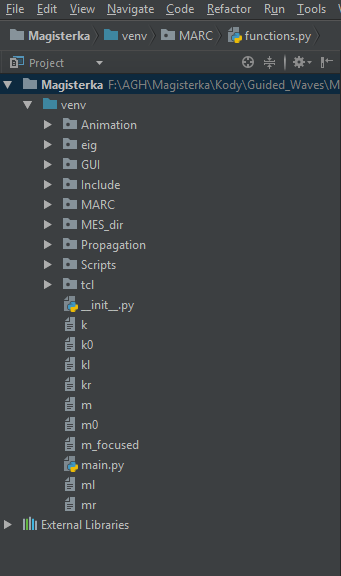
\includegraphics[width=8cm]{Zdjecia/5/okno_projektu}
\caption{Widok okna projektu}
\label{fig:okno_projektu}
\end{figure}


\subsection{Elementy czworościenne}
\label{cha:elementy czworościenne}

Zawartość katalogu MES dir przedstawia rysunek \ref{fig:okno_projektu_MES}. Obliczenia dotyczące elementów czworościennych zawarte są w modułach katalogu tetrahedralElements. Poniżej znajdują się funkcje poszczególnych modułów, wraz z opisem ich zastosowania, argumentami wejściowymi oraz wyjściowymi.

Dane zbierane w postaci macierzy są najczęściej tablicami array z biblioteki NumPy, która służy do obliczeń numreycznych. W części modułów obliczenia są prowadzone na zmiennych symbolicznych z wykorzystaniem biblitoeki SymPy. Macierze zmiennych symbolicznych są obiektami Matrix z tej biblioteki.

\begin{figure}[h]
\centering
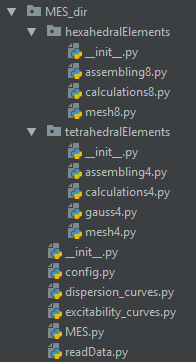
\includegraphics[width=5cm]{Zdjecia/5/okno_projektu_MES}
\caption{Zawartość katalogu MES\_dir}
\label{fig:okno_projektu_MES}
\end{figure}

\vspace {3mm}
 \( \textbf{Moduł mesh4} \).

\vspace {3mm}
\textit{circlePlaneVerticies(x, radius, numberOfPoints)} - funkcja wykorzystywana przy tworzeniu siatki (w circleMeshFull oraz circleMeshSparse). Dodaje do siatki węzły na okręgu w jednej płaszczyźniej pręta, która znajduje się na długości x. Promień okręgu określa - radius, a ilość węzłów na okręgu - numberOfPoints.

\vspace {3mm}
\textit{circleMeshFull(radius, numberOfCircles, numberOfPoints)} - funkcja tworzy siatkę na trzech płaszczyznach przesuniętych o 1 we współrzędnej x. Siatka zbudowana jest na każdej płaszczyźnie tak samo i zawiera węzeł centralny oraz okręgi z węzłami w ilości numberOfCircles. Na każdym okręgu liczba węzłów jest większa, aby zapewnić możliwie równe odległości pomiędzy węzłami. Pierwszy okrąg zawiera liczbę węzłów numberOfPoints. Zwraca tablicę o wymiarach n x 3, gdzie n to liczba węzłów. W kolumnach są kolejne współrzędne węzłów.

\vspace {3mm}
\textit{circleMeshSparse(radius, numberOfCircles, numberOfPoints)} - jak wyżej, z tą różnicą, że każdy okrąg siatki ma tyle samo węzłów.

\vspace {3mm}
\textit{triangulation(vertices)} - funkcja tworzy elementy skończone czworościenne. Przyjmuje macierz węzłów z powyższych funkcji - vertices i zwraca tablicę e x 4, gdzie e to liczba elementów. W kolumnach zawarte są indeksy węzłów z macierzy wejściowej, które należą do danego elementu.

\vspace {3mm}
\textit{correctVolumeSign(vertices, indices)} - funkcja przyjmuje macierz współrzędnych węzłów - vertices oraz indeksy węzłów dla każdego elementu skończonego - indices. Sprawdza czy objętość elementu skończonego obliczona za pomocą wyznacznika ma dodatnią wartość. Jeśli nie, to zmienia miejscami dwa indeksy elementu w macierzy zwróconej z triangulation(vertices).

\vspace {3mm}
\textit{drawPlane(vertices)} - funkcja przyjmuje macierz współrzędnych węzłów - vertices i rysuje ich układ na płaszczyźnie. Przykładowe układu przedstawione są na rysunku \ref{fig:siatka}.

\vspace {3mm}
\textit{drawBar(vertices)} - funkcja przyjmuje macierz współrzędnych węzłów - vertices i rysuje wszystkie węzły w rzucie izometrycznym. Przykład przedstawia rysunek \ref{fig:pret}.

\vspace {3mm}
\textit{drawTriangulation(vertices, indices)} - funkcja przyjmuje macierz współrzędnych węzłów - vertices i macierz elementów skończonych - indices. Rysuje elementy skończone w rzucie izometrycznym. Przykład przedstawia rysunek \ref{fig:triangulation}.

\begin{figure}
\begin{subfigure}{.5\textwidth}
  \centering
  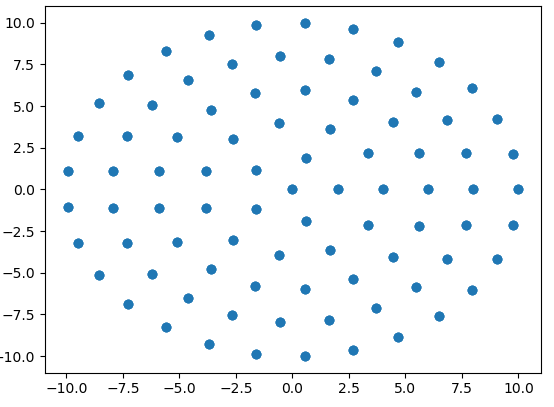
\includegraphics[width=.8\linewidth]{Zdjecia/5/siatka1}
  \caption{}
  \label{fig:sfig1}
\end{subfigure}%
\begin{subfigure}{.5\textwidth}
  \centering
  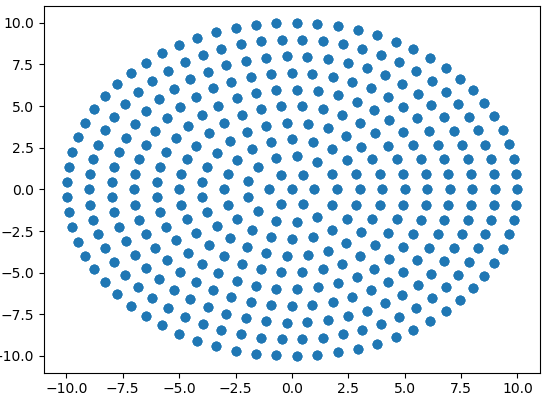
\includegraphics[width=.8\linewidth]{Zdjecia/5/siatka2}
  \caption{}
  \label{fig:sfig2}
\end{subfigure}\\
\begin{subfigure}{.5\textwidth}
  \centering
  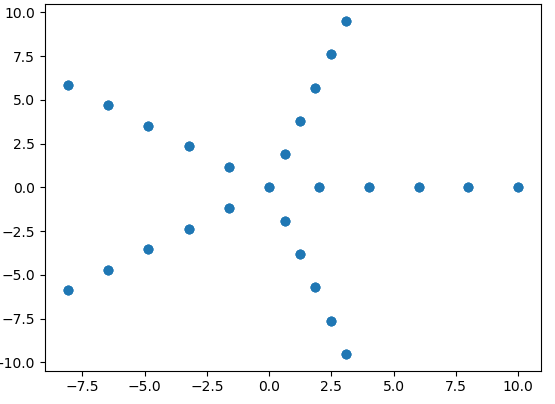
\includegraphics[width=.8\linewidth]{Zdjecia/5/siatka3}
  \caption{}
  \label{fig:sfig3}
\end{subfigure}%
\begin{subfigure}{.5\textwidth}
  \centering
  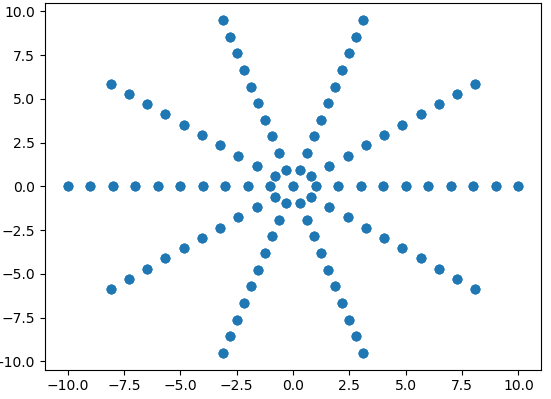
\includegraphics[width=.8\linewidth]{Zdjecia/5/siatka4}
  \caption{}
  \label{fig:sfig4}
\end{subfigure} 
\caption{Układ siatki węzłów na płaszczyźnie powstałych z a) \textit{circleMeshFull(10, 5, 5)} b) \textit{circleMeshFull(10, 10, 10)} c) \textit{circleMeshSparse(10, 5, 5)} d) \textit{circleMeshSparse(10, 10, 10)}}
\label{fig:siatka}
\end{figure}


\begin{figure}
\begin{subfigure}{.5\textwidth}
  \centering
  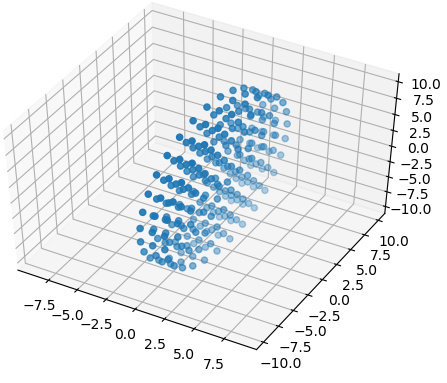
\includegraphics[width=.8\linewidth]{Zdjecia/5/pret1}
  \caption{}
  \label{fig:sfig1}
\end{subfigure}%
\begin{subfigure}{.5\textwidth}
  \centering
  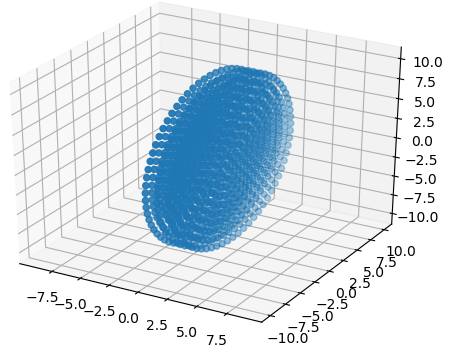
\includegraphics[width=.8\linewidth]{Zdjecia/5/pret2}
  \caption{}
  \label{fig:sfig2}
\end{subfigure}\\
\begin{subfigure}{.5\textwidth}
  \centering
  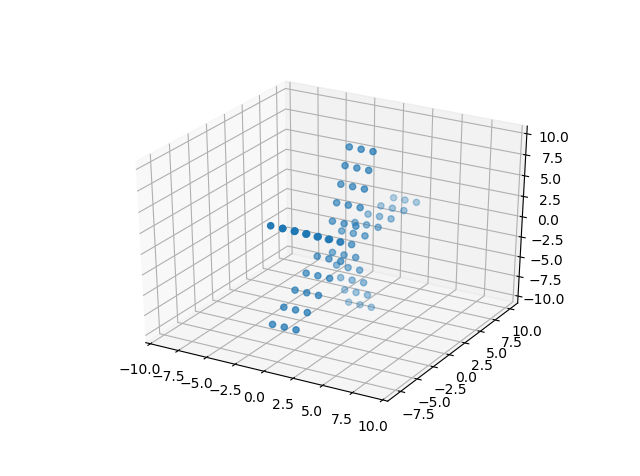
\includegraphics[width=.8\linewidth]{Zdjecia/5/pret3}
  \caption{}
  \label{fig:sfig3}
\end{subfigure}%
\begin{subfigure}{.5\textwidth}
  \centering
  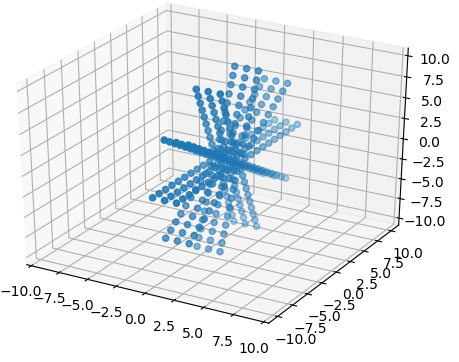
\includegraphics[width=.8\linewidth]{Zdjecia/5/pret4}
  \caption{}
  \label{fig:sfig4}
\end{subfigure} 
\caption{Układ siatki węzłów pręta z a) \textit{circleMeshFull(10, 5, 5)} b) \textit{circleMeshFull(10, 10, 10)} c) \textit{circleMeshSparse(10, 5, 5)} d) \textit{circleMeshSparse(10, 10, 10)}}
\label{fig:pret}
\end{figure}

\begin{figure}
\begin{subfigure}{.5\textwidth}
  \centering
  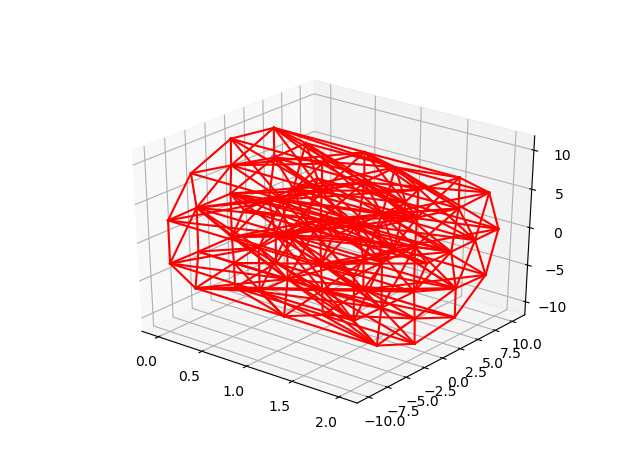
\includegraphics[width=.8\linewidth]{Zdjecia/5/triangulation1}
  \caption{}
  \label{fig:sfig1}
\end{subfigure}%
\begin{subfigure}{.5\textwidth}
  \centering
  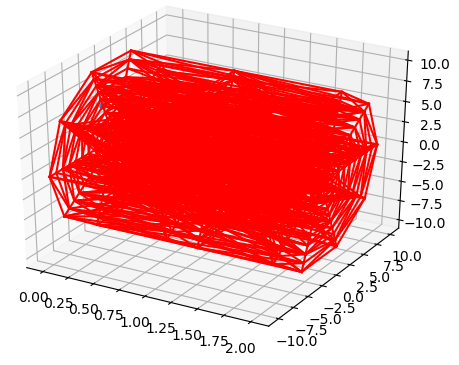
\includegraphics[width=.8\linewidth]{Zdjecia/5/triangulation2}
  \caption{}
  \label{fig:sfig2}
\end{subfigure}

\caption{Triangulacja (elementy skończone) dla siatki a) \textit{circleMeshFull(10, 3, 3)} b) \textit{circleMeshSparse(10, 10, 10)}}
\label{fig:triangulation}
\end{figure}

\vspace {3mm}
 \( \textbf{Moduł calculation4} \).

\vspace {3mm}
\textit{pVector()} - funkcja zwraca macierz zmiennych symbolicznych z wektorem p dla elementu czworościennego.

\vspace {3mm}
\textit{meMatrix(vertices, elementIndices)} - funkcja przyjmuje macierz współrzędnych węzłów - vertices oraz indeksy dla węzłów elementu skończonego - elementIndices i zwraca macierz \( M^e \).

\vspace {3mm}
\textit{meInvMatrix(vertices, elementIndices)} - jak powyżej, dodatkowo macierz wyjściowa jest odwrócona w stosunku do poprzedniej funkcji.

\vspace {3mm}
\textit{shapeFunctions(vertices, elementIndices)} - funkcja przyjmuje macierz współrzędnych węzłów - vertices i indeksy dla węzłów elementu skończonego - elementIndices, a zwraca funkcje kształtu w formie tablicy zmiennych symbolicznych.

\vspace {3mm}
\textit{bMatrixFc(shapeFunctions)} - funkcja przyjmuje tablicę funkcji kształtu w postaci symbolicznej - shapeFunctions, a zwraca macierz B w postaci tablicy numerycznej. Funkcje kształtu są dla elementów czworościennych liniowe więc ich pochodne są stałymi. 

\vspace {3mm}
\textit{bMatrixNatural(shapeFunctions)} - jak powyżej, ale dla tablicy funkcji kształtu we współrzędnych naturalnych.

\vspace {3mm}
\textit{dMatrixFc(youngModulus, poissonCoeficient)} - funkcja zwraca macierz D, obliczoną na podstawie modułu Younga - youngModulus oraz współczynnik Poissona - poissonCoeficient.

\vspace {3mm}
\textit{stiffLocalMatrix(shapeFunctions, vertices, elementIndices, youngModulus, poissonCoefficient)} - funkcja przyjmuje jako argumenty funkcje kształtu w formie symbolicznej - shapeFunctions, macierz współrzędnych węzłów - vertices, indeksy węzłów elementu skończonego - element indices oraz moduł Younga - youngModulus i współczynnik Poissona - poissonCoeficient. Zwraca macierz sztywności dla elementu skończonego.

\vspace {3mm}
\textit{massLocalMatrix(density)} - funkcja przyjmuje gęstość materiału - density. Zwraca macierz mas obliczoną we współrzędnych naturalnych bez uwzględnienia jakobianu. Na tym etapie nie jest to więc poprawnie wyznaczona macierz mas. Jakobian jest stały dla elementów czworościennych i uwzględniany jest na etapie agregacji. Pozwala to obliczyć całkę \ref{eq:macierz_mas} bez uwzględnienia jakobianu raz, a następnie mnożyć ją dla każdego elementu przez jakobian.

\vspace {3mm}
\textit{volume(elementVertices)} - funkcja przyjmuje współrzędne węzłów elementu - elementVertices i oblicza objętość elementu z wykorzystaniem geometrii analitycznej.

\vspace {3mm}
\textit{volumeDet(vertices)} - jak powyżej z tym, że objętość jest obliczano za pomocą wyznacznika macierzy \( M^e \).

\vspace {3mm}
 \( \textbf{Moduł gauss4} \).
Moduł zawiera funkcje pomocnicze do całkowania macierzy mas. Obliczanie macierzy sztywności nie wymaga całkowania, ponieważ macierz B jest stała.

\vspace {3mm}
\textit{shapeFunctionsNatural()} - zwraca tablicę funkcji kształtu we współrzędnych naturalnych, w formie symbolicznej.

\vspace {3mm}
\textit{coordinateChangeModel(elementVertices, naturalShapeFc)} - funkcja przyjmuje funkcje kształtu we współrzędnych naturalnych - naturalShapeFc  oraz współrzędne węzłów elementu skończonego - elementVertices i oblicza zależność współrzędnych rzeczywistych i naturalnych. Zwraca trzy wyrażenia symboliczne zawierające współrzędne naturalne. Przedtsawiają one współrzędne rzeczywiste, kolejno x, y, z.

\vspace {3mm}
\textit{jacobian(elementVertices, naturalShapeFc)} - funkcja przyjmuje współrzędne węzłów elementu skończonego - elementVertices oraz funkcje kształtu we współrzędnych naturalnych - naturalShapeFc. Zwraca jakobian przekształcenia, który jest wykorzystywany w obliczaniu macierzy mas.

\vspace {3mm}
\textit{matrixToIntegrate(density)} - funkcja przyjmuje gęstość materiału - density. Zwraca macierz podcałkową, do obliczania macierzy mas. Nie uwzględnia jakobianu, który jest stały. Wynik całkowania jest mnożony przez jakobian na etapie agregacji.

\vspace {3mm}
 \( \textbf{Moduł assembling4} \).
Moduł zawiera funkcje do obliczania macierzy globalnych. Pozwala też na wizualizację rzadkości macierzy.

\vspace {3mm}
\textit{assembleGlobalStiffMatrix(vertices, indices, youngModulus, poissonCoefficient)} - funkcja przyjmuje macierz współrzędnych węzłów konstrukcji - vertices, indeksy wszystkich elementów - indices, moduł Younga - youngModulus i współczynnik Poissona - poissonCoeficient. Zwraca globalną macierz sztywności.

\vspace {3mm}
\textit{drawMatrixSparsity(matrix)} - funkcja przyjmuje macierz - matrix. Pozwala rysować rzadkość macierzy w postaci bitmapy, gdzie każdy element macierzy jest jednym pikselem.

\vspace {3mm}
\textit{assembleGlobalMassMatrix(vertices, indices, density)} - funkcja przyjmuje macierz współrzędnych węzłów konstrukcji - vertices, indeksy węzłów wszystkich elementów skończonych - indices oraz gęstość materiału - density. Zwraca globalną macierz mas.

\vspace {3mm}
\textit{focuseMatrixRows(matrix)} - funkcja przyjmuje macierz - matrix. Zwraca macierz skupioną poprzez sumowanie elementów w wierszu i umieszczanie ich na diagonali. Wykorzystywana przy obliczeniach ze skupioną macierza mas.



\subsection{Elementy sześcienne}
\label{cha:elementy szescienne}

Obliczenia dotyczące elementów sześciennych zawarte są w modułach katalogu hexahedralElements. Poniżej znajdują się funkcje poszczególnych modułów, wraz z opisem ich zastosowania, argumentami wejściowymi oraz wyjściowymi.

 \( \textbf{Moduł mesh8} \).

\vspace {3mm}
\textit{circleMeshFull(radius, firstCircle, addNodes, circles)} - funkcja działa jak funcja z modułu mesh4 z tą różnicą, że przyjmuje dodatkowy argument addNodes. Określa on ile punktów więcej ma być na każdym kolejnym okręgu siatki.

\vspace {3mm}
\textit{circleMeshSparse(radius, firstCircle, circles)} - funkcja działa jak odpowiednik z modułu mesh4

\vspace {3mm}
\textit{createFiniteElements(vertices, pointsOnLastCircle, length, numberOfPlanes)} - funkcja przyjmuje jako argumenty macierz współrzędnych węzłów, liczbę punktów na ostatnim okręgu siatki, długość modelu pręta oraz liczbę płaszczyzn siatki. Tworzy elementy sześcienne w kilku etapach. Najpierw jedna z płaszczyzn dzielona jest na trójkąty. Następnie trójkąty są łączone w pary i w ten sposób powstają czworokąty. W większości konfiguracji siatki na brzegach pozostają puste miejsca z trójkątów, które nie mają pary. W takich miejscach dodawany jest dodatkowy punkt siatki i z trójkąta tworzony czworokąt. Następnie identyczne czworokąty są tworzone na kolejnych płaszczyznach i wzdłuż długości pręta tworzone są z nich sześciościany. Zwraca macierz e x 8, gdzie e to liczba elementów skończonych. W kolumnach są indeksy kolejnych punktów siatki.

\vspace {3mm}
\textit{brickMesh(radius, numberOfPlanes, numberOfCircles, numberOfPointsOnCircle)} - funkcja tworzy siatkę o kształcie wielokąta na pierwszym okręgu. Przyjmuje jako argumenty promień - radius, liczbę płaszczyzn siatki - numberOfPlanes, liczbę okręgów na płaszczyźnie siatki - numberOfCircles oraz ilość wierzchołków wielokąta wpisanego w okrąg - numberOfPointsOnCircle. Zwraca tablicę o wymiarach n x 3, gdzie n to liczba węzłów. W kolumnach są kolejne współrzędne węzłów.

\vspace {3mm}
\textit{createBrickElements(brickVertices, numberOfPlanes, numberOfCircles, numberOfPointsOnCircle)} - funkcja przyjmuje macierz współrzędnych węzłów z funkcji \textit{brickMesh} - brickVertices, liczbę płaszczyzn siatki - numberOfPlanes, liczbę okręgów na każdej płaszczyźnie - numberOfCircles oraz liczbę wierzchołków wielokąta wpisanego w każdy okrąg - numberOfPointsOnCircle. Tworzy elementy sześciościenne na zadanej siatce. Zwraca macierz e x 8, gdzie e to liczba elementów skończonych. W kolumnach są indeksy kolejnych punktów siatki.

\vspace {3mm}
\textit{drawPlane(vertices)} - jak w mesh4. Przykładowe siatki z tego modułu są przedstawione na rysunku \ref{fig:hex_siatka}.

\vspace {3mm}
\textit{drawBar(vertices)} - jak w mesh4

\vspace {3mm}
\textit{drawTetragons(vertices, indices)} - funkcja przyjmuje jako argumenty macierz współrzędnych węzłów - vertices oraz macierz indeksów węzłów dla każdego elementu - indices. Rysuje układ czworokątów na płaszczyźnie. Przykłady są przedstawione na rysunku \ref{fig:hex_czworokaty}.

\vspace {3mm}
\textit{drawHexahedrons(vertices, indices)} - funkcja przyjmuje jako argumenty macierz współrzędnych węzłów - vertices oraz macierz indeksów węzłów dla każdego elementu - indices. Rysuje model złożony z sześciościanów w rzucie izometrycznym. Przykład znajduje się na rysunku \ref{fig:hex_elementy}.

\begin{figure}
\begin{subfigure}{.5\textwidth}
  \centering
  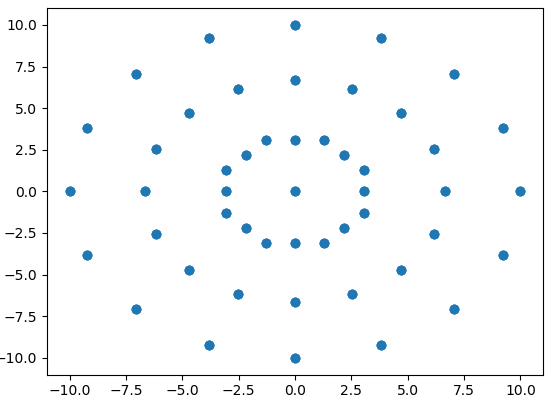
\includegraphics[width=1.0\linewidth]{Zdjecia/5/hex_siatka1}
  \caption{}
  \label{fig:sfig1}
\end{subfigure}
\begin{subfigure}{.5\textwidth}
  \centering
  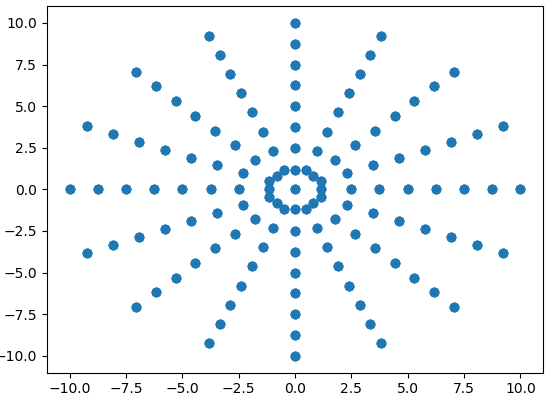
\includegraphics[width=1.0\linewidth]{Zdjecia/5/hex_siatka2}
  \caption{}
  \label{fig:sfig2}
\end{subfigure}
\caption{Układ siatki węzłów na płaszczyźnie powstałych z a) \textit{brickMesh(10, 3, 3, 16)} b) \textit{brickMesh(10, 3, 8, 16)} }
\label{fig:hex_siatka}
\end{figure}

\begin{figure}
\begin{subfigure}{.5\textwidth}
  \centering
  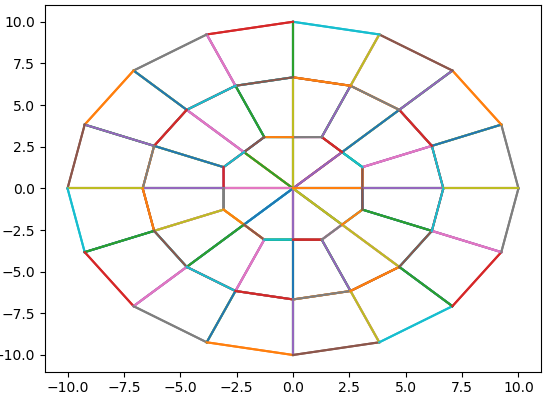
\includegraphics[width=1.0\linewidth]{Zdjecia/5/hex_czworokaty1}
  \caption{}
  \label{fig:sfig1}
\end{subfigure}
\begin{subfigure}{.5\textwidth}
  \centering
  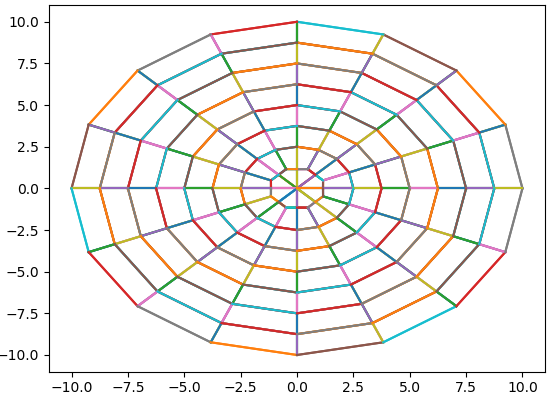
\includegraphics[width=1.0\linewidth]{Zdjecia/5/hex_czworokaty2}
  \caption{}
  \label{fig:sfig2}
\end{subfigure}
\caption{Czworokąty będące ścianą elementu skończonego na płaszczyźnie a) \textit{brickMesh(10, 3, 3, 16)} b) \textit{brickMesh(10, 3, 8, 16)} }
\label{fig:hex_czworokaty}
\end{figure}

\begin{figure}
\begin{subfigure}{.5\textwidth}
  \centering
  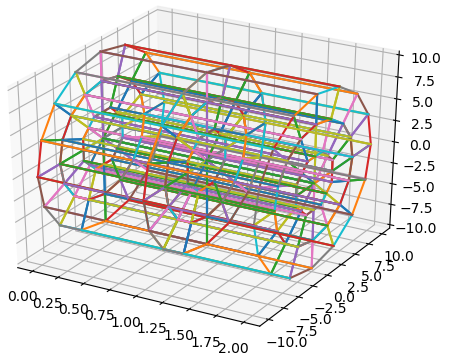
\includegraphics[width=1.0\linewidth]{Zdjecia/5/hex_elementy1}
  \caption{}
  \label{fig:sfig1}
\end{subfigure}
\begin{subfigure}{.5\textwidth}
  \centering
  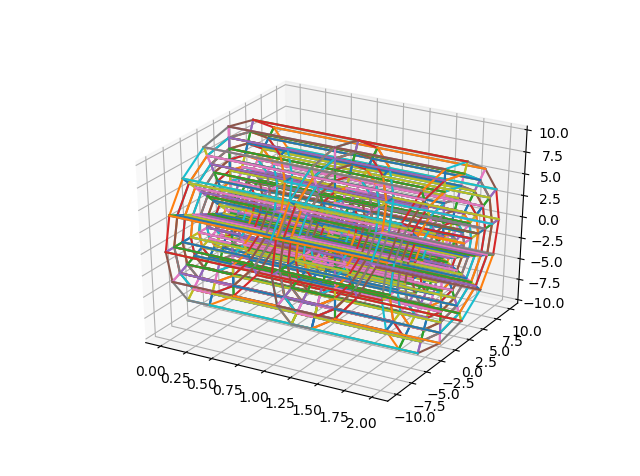
\includegraphics[width=1.0\linewidth]{Zdjecia/5/hex_elementy2}
  \caption{}
  \label{fig:sfig2}
\end{subfigure}
\caption{Elementy skończone zbudowane na siatce a) \textit{brickMesh(10, 3, 3, 16)} b) \textit{brickMesh(10, 3, 8, 16)} }
\label{fig:hex_elementy}
\end{figure}

\vspace {3mm}
 \( \textbf{Moduł calculations8} \).

\vspace {3mm}
\textit{localStiffMatrix(elementVertices)} - funkcja przyjmuje jako argumenty macierz współrzędnych węzłów elementu skończonego. Zwraca macierz sztywności elementu skończonego.

\vspace {3mm}
\textit{localMassMatrix(elementVertices)} - funkcja przyjmuje jako argumenty macierz współrzędnych węzłów elementu skończonego - elementVertices. Zwraca macierz mas elementu skończonego.

\vspace {3mm}
 \( \textbf{Moduł assembling8} \).

\vspace {3mm}
\textit{assembleGlobalStiffMatrix(vertices, indices)} - funkcja przyjmuje jako argument macierz współrzędnych węzłów konstrukcji - vertices oraz macierz indeksów węzłów elementów skończonych - indices. Zwraca macierz sztywności konstrukcji.

\vspace {3mm}
\textit{assembleGlobalMassMatrix(vertices, indices)} - funkcja przyjmuje jako argument macierz współrzędnych węzłów konstrukcji - vertices oraz macierz indeksów węzłów elementów skończonych - indices. Zwraca macierz mas konstrukcji.

\vspace {3mm}
\textit{focuseMatrixRows(matrix)} - funkcja przyjmuje macierz - matrix. Zwraca macierz skupioną poprzez sumowanie elementów w wierszu i umieszczanie ich na diagonali. Wykorzystywana przy obliczeniach ze skupioną macierza mas.

\vspace {3mm}
\textit{drawMatrixSparsity(matrix)} - funkcja przyjmuje macierz - matrix. Pozwala rysować rzadkość macierzy w postaci bitmapy, gdzie każdy element macierzy jest jednym pikselem.


\subsection{Pozostałe moduły katalogu MES\_dir}
\label{cha:pozostale_moduly}

 \( \textbf{Moduł config} \).

W tym module przechowywane są dane wykorzystywane w innych częściach programu. Jego zawartość podana jest poniżej.

\vspace {3mm}
ROOT\_DIR = os.path.dirname(os.path.abspath(\_\_file\_\_))

\#sciezka do katalogu MES\_dir
\vspace {3mm}
ndof = 3    \# liczba stopni swobody

kvect\_min = 0

kvect\_no\_of\_points = 0

kvect\_max = 2*pi
\vspace {3mm}
k = []  \# globalna macierz sztywnosci

m = []  \# globalna macierz mas

m\_focused\_rows = [] \#globalna macierz mas - skupiona wierszami

ml = []

m0 = []

mr = []

kl = []

k0 = []

kr = []
\vspace {3mm}
force = []
\vspace {3mm}
\# Stale materialowe

young\_mod = 70000

poisson\_coef = 0.3

density = 2.7*1e-9
\vspace {3mm}
\# Wyswietlanie siatki na plaszczyznie, siatki w 3D i triangulacji

show\_plane = False

show\_bar = False

show\_elements = False

saveEigVectors = False
\vspace {3mm}

Pierwszym elementem jest ścieżka do katalogu pozwalająca wygodnie odnosić się do niego w funkcjach zapisujących i wczytujących dane z plików. Poniżej znajdują się wartość minimalna, maksymalna oraz liczba próbek wartości liczby falowej, dla których to wartości obliczane będą częstości własne. Następnie kolejno zawarte są macierze i podmacierze modelu MES, siła wymuszająca wykorzystywana przy obliczaniu wzbudzalności, stałe materiałowe konstrukcji pręta i wartości logiczne określające czy wyświetlać siatkę lub element skończone modelu.

\vspace {3mm}

 \( \textbf{Moduł MES} \).
W tym module zawarte są dwie funkcje, które są przykładami budowy modelu za pomocą elementów czworościennych oraz sześciościennych.

\textit{mes4(radius, numOfCircles, numOfPointsAtFirstCircle)} - funkcja przyjmuje jako argumenty promień pręta - radius, liczbę okręgów na jednej płaszczyźnie siatki - numOfCircles oraz liczbę węzłów na pierwszym okręgu siatki - numOfPointsAtFirstCircle. Poniżej znajduje się całość kodu tej funkcji.

\vspace {3mm}

    vertices = mesh4.circleMeshFull(radius, numOfCircles, numOfPointsAtFirstCircle)

    if config.show\_plane:

        mesh4.drawPlane(vertices)

    if config.show\_bar:

        mesh4.drawBar(vertices)

\vspace {3mm}
    indices = mesh4.triangulation(vertices)

    \# mesh.draw\_triangulation(vertices, indices)

    if config.show\_elements:

        mesh4.drawTriangulation(vertices, indices)

\vspace {3mm}
    start = time.clock()

    config.k = assembling4.assembleGlobalStiff\_matrix(vertices, indices, config.young\_mod, config.poisson\_coef)

    \# assembling.drawMatrixSparsity(config.k)

    print("Macierz sztywnosci gotowa")

    print("Wykonywanie: ", time.clock() - start)

\vspace {3mm}
    config.m = assembling4.assembleGlobalMassMatrix(vertices, indices, config.density)

    config.m\_focused\_rows = assembling4.focuseMatrixRows(config.m)

    \# assembling.drawMatrixSparsity(config.m)

    print("Macierz mas gotowa")

    print("wykonywanie: ", time.clock() - start)

\vspace {3mm}

W pierwszej lini uzyskiwana jest macierz współrzędnych węzłów siatki. Następnie siatka jest wyświetlana w na płaszczyźnie, bądź w rzucie izometrycznym jeśli wartości z modułu config mają wartości TRUE. Kolejnym etapem jest tworzenie elementów skończonych i warunkowe ich wyświetlanie. Wartość start przechowuje czas, w którym rozpoczyna się obliczanie macierzy sztywności - k. Po obliczeniu tej macierzy wyświetlany jest komunikat z czasem obliczeń.  Podobnie poniżej w przypadu macierzy mas.

\textit{mes8(numberOfPlanes, radius, numberOfCircles, numberOfPointsOnCircle, addNodes)} - funkcja przyjmuje jako argumenty liczbę płaszczyzn siatki - numberOfPlanes, promień pręta - radius, liczbę okręgów na jednej płaszczyźnie siatki - numOfCircles, liczbę węzłów na pierwszym okręgu siatki - numOfPointsOnCircle oraz liczbę dodatkowych punktów na każdym kolejnym okręgu siatki przy zastosowaniu odpowiedniego jej typu - addNodes. Poniżej znajduje się całość kodu tej funkcji.

\vspace {3mm}
    \# brickMesh(radius, numberOfPlanes, numberOfCircles, numberOfPointsOnCircle)

    vertices = mesh8.brickMesh(radius, numberOfPlanes, numberOfCircles, numberOfPointsOnCircle)

    \# createBrickElements(brickVertices, numberOfPlanes, numberOfCircles, numberOfPointsOnCircle)

    indices = mesh8.createBrickElements(vertices, 3, 3, 16)

\vspace {3mm}
    start = time.clock()

    config.k = assembling8.assembleGlobalStiffMatrix(vertices, indices)

    print("Macierz sztywnosci gotowa")

    print("Wykonywanie: ", time.clock() - start, " [s]")

    print("Wykonywanie: ", (time.clock() - start)/3600, " [h]")

    start = time.clock()

\vspace {3mm}
    config.m = assembling8.assembleGlobalMassMatrix(vertices, indices, config.density)

    config.m\_focused\_rows = assembling8.focuse\_matrix\_rows(config.m)

    print("Macierz mas gotowa")

    print("wykonywanie: ", time.clock() - start, " [s]")

    print("wykonywanie: ", (time.clock() - start)/3600, " [h]")

\vspace {3mm}
W tym przykładzie zastosowano siatkę brickMesh. Po wyznaczeniu współrzędnych węzłów oraz zbudowaniu elementów skończonych, obliczane są macierze mas i sztywności.

 \( \textbf{Moduł dispersion\_curves} \).
W tym module wyznaczone są punkty krzywych dyspersji, na podstawie macierzy mas i sztywności wyznaczonych z modelu MES.

\vspace {3mm}
\textit{getDataForEiq()} - funkcja wyznacza podmacierze mas i sztywności potrzebne do zastosowania wzoru \ref{eq:MES5}. Macierze przechowywane są w module \textit{config}. Dodatowo po wyznaczeniu zapisywane są do plików tekstowych, tak więc nie ma potrzeba wyznaczania ich ponownie w celu innego wykorzystania.

\vspace {3mm}
\textit{findEig()} - funkcja dla kolejnych wartości liczby falowej oblicza wartości i wektory własne pary macierzy, wyznaczonych jak we wzorze \ref{eq:MES5}. Dodatkowo wektory własne zapisywane są w niej do pliku.

\vspace {3mm}
\textit{drawDispercionCurves(number\_of\_curves\_to\_draw=10, save\_plot\_to\_file=False)} - funkcja przyjmuje jako argument liczbę początkowych modów do wyświetlenia - number\_of\_curves\_to\_draw oraz wartość logiczną określająca czy zapisać wykres do pliku png - save\_plot\_to\_file. Dodatkowo zapisauje wszystkie wartości własne w pliku tesktowym.

\vspace {3mm}
\textit{drawDispercionCurvesFromFile(number\_of\_curves\_to\_draw=10, save\_plot\_to\_file=False)} - jak powyżej z tym, że funkcja ta służy do rysowania krzywych dyspersji z wartości wczytywanych z plików tekstowych.

\vspace {3mm}
\textit{sortColumns(matrix)} - funkcja służy do wstępnego sortowania wartości własnych. Sortuje je kolumnami od najmniejszej do największej. W każdej kolumnie zapisane są wartości własne dla jednej wartości liczby falowej. Sortowanie takie jest więc poprawne tylko dla modów początkowych, które się nie krzyżują. Bardziej zaawansowany algorytm sortowania jest wprowadzany na etapie obliczeń związanym z wykorzystywaniem krzywych dyspersji.
%
%\vspace {3mm}
% \( \textbf{Moduł excitabiliti\_curves} \).
%Moduł pozwala na obliczanie krzywych wzbudzalności dla poszczególnych modów. 
%
%\vspace {3mm}
%\textit{hermitianTranspose(matrix)} - funkcja przyjmuje jako argument macierz, a zwraca sprzężenie hermitowskie macierzy wejściowej.
%
%\vspace {3mm}
%\textit{calculateP(kr, kl, wavenumber, eigvector)} - funcja przyjmuje jako argumenty podmacierze macierzy sztywności \( k\_r \) i \(k\_l \) wykorzystywane wcześniej we wzorze \ref{eq:MES5}, wartości liczby falowej, dla których wyznaczano wartości i wektory własne - wavenumber oraz wektory własne - eigvector. Zwraca wartość \( P \) zgodnie ze wzorem \ref{eq:wzbudzanie3}.
%
%\vspace {3mm}
%\textit{calculateExcitablity(mode, f)} - funkcja przyjmuje jako argumenty numer modu - mode oraz wektor będący wymuszającą siłą węzłową dla modelu MES - f. Wyznacza dla każdej częstotliwości, z którą związany jest wektor własny, wartość amplitudy. Zwraca wektor częstotliwości i amplitudy.
%
%\vspace {3mm}
%\textit{calculateAndShowCurves(numberOfModes)} - funkcja przyjmuje jako argument liczbę początkowych modów, dla których ma wyznaczyć krzywe wzbudzalności- numberOfModes. Po obliczeniu przedstawia wykres krzywych wzbudzalności.


\vspace {3mm}
 \( \textbf{Moduł singi\_around} \).
Moduł pozwala na symulację efektu sing around.

\vspace {3mm}
\textit{getSignalSpectrum()} - funkcja generuje sygnał, którego symulacja będzie symulowana. W tym przypadku jest to sygnał chirp.

\vspace {3mm}
\textit{getCurvesInSignalArgs(numberOfModes, args)} - funcja przyjmuje jako argumenty liczbę modów - numberOfModes oraz argumenty widma badanego sygnału - args. Pozwala na znalezienie wartości liczby falowej oraz amplitudy dla krzywych, dla częstotliwości zawartych w widmie badanego sygnału. Zwraca macierze liczby falowej i amplitudy z liczbą wierszy równa liczbie modów, oraz liczbą kolumn równą liczbie punktów sygnału badanego.

\vspace {3mm}
\textit{lenghtPropagate(length, fChirp, kvect, excAmplitude)} - funcja przyjmuje jako argumenty długość ścieżki propagacji - length, widmo badanego sygnału - fChirp, macierz liczb falowych związanych z krzywymi dyspersji - kvect oraz macierz amplitud krzywych wzbudzalności - excAmplitude. Przyjmowane macierze są obliczone tak, że wartości wyznaczone w tych samych częstościach, w których znajdują się wartości sygnału chirp. Funkcja zwraca widmo sygnału po propagacji na wprowadzonej długości.

\vspace {3mm}
\textit{singAround(iterations, length, frequency, fChirp, kvect, excAmplitude)} - funkcja przyjmuje jako argumenty liczbę cykli propagacji - iterations, długość ścieżki propagacji - length, częstotliwości zawarte w sygnale - frequency, widmo sygnału - fChirp, macierz liczb falowych - kvect oraz macierz amplitud krzywych wzbudzalności - excAmplitude. Funkcja zwraca widmo sygnału po kilkukrotnej propagacji na zadanej długości.

\vspace {3mm}
\textit{plotSignal(args, values)} - funkcja przyjmuje jako argumenty wektor argumentów funkcji - args oraz wektor wartości funkcji - values. Rysuje zadaną funkcję.

\vspace {3mm}
\textit{plotCurves(args, values)} - funkcja przyjmuje jako argumenty wektor argumentów funkcji - args oraz macierz wartości funkcji dla kilku krzywych - values. Rysuje zadane krzywe.

\vspace {3mm}
 \( \textbf{Moduł readData} \).
W tym module zawarte są wszystkie funkcje służące do zapisu i wczytywania danych. Nie będą one z osobna omawiane ponieważ ich funkcja jest jasna. Poniżej omówiony jest sposób umieszczania danych w plikach.

Wszystkie dane umieszczone są w katalogu \textit{eig}. Liczby falowe zapisane są w pliku \textit{kvect}. Każda wartość znajduje się w osobnej lini.

Wartości własne zapisane są w pliku \textit{omega}. Każda kolumna zawiera wartości własne wyznaczone dla jednej wartości liczby falowej.

Wektory własne zapisywane są w katalogu \textit{eig}, w plikach mających w nazwie \textit{eig\_}, a następnie wartość liczby falowej. W każdym z takich plików zapisane są wartości własne i odpowiadające im wektory własne dla jednej wartości liczby falowej. W pierwszej linii znajduje się wartość własna, w drugiej odpowiadający jej wektor własny, a następnie pozostałe wartości i wektory własne w kolejnych liniach.

\subsection{Moduł main}
\label{cha:main}

Przykładowy skrypt wyznaczający krzywe dyspersji, z pomocą wcześniej opisanych modułów, znajduje się w module \textbf{main} głównego katalogu projektu. Kod przedstawiony jest poniżej.

\vspace{3mm}
import sympy as sp

import numpy as np

from MES\_dir import MES, config, dispersion\_curves

from MARC import functions

\vspace{3mm}
\# begin MES

x, y, z = sp.symbols('x, y, z')

if \_\_name\_\_ == "\_\_main\_\_":

\vspace{3mm}
    print("Wpisz wartość: ")

    print("1 - rysowanie krzywy dyspersji z wykorzystaniem MES")

    print("2 - rysowanie krzywych dyspersji z ostatnio policzonych danych")

    text = input()

\vspace{3mm}
    if text == '1':

\vspace{3mm}
        print("Wpisz wartość: ")

        print("4 - elementy czworościenne")

        print("8 - elemnty sześcienne")

        print("M - wczytanie macierzy z MARC i wykreślenie krzywych")

        text1 = input()

\vspace{3mm}
        \# wektor liczby falowej

        config.kvect\_min = 1e-10

        config.kvect\_max = np.pi / 4

        config.kvect\_no\_of\_points = 51

\vspace{3mm}
        \# rysowanie wykresow

\vspace{3mm}
        config.show\_plane = True

        config.show\_bar = True

        config.show\_elements = True

\vspace{3mm}

        \# zapisywanie wektorow wlasnych
        saveEigVectors = True

\vspace{3mm}
        \# obliczenia

        if text1 == '4':

            \# parametry preta

            radius = 10

            num\_of\_circles = 4

            num\_of\_points\_at\_c1 = 4

            MES.mes4(radius, num\_of\_circles, num\_of\_points\_at\_c1)

\vspace{3mm}

        if text1 == '8':

            radius = 10

            numberOfPlanes = 3

            firstCircle = 16 \#for brickMesh should be 16

            addNodes = 0

            circles = 1

            MES.mes8(numberOfPlanes, radius, circles, firstCircle, addNodes)

\vspace{3mm}
        if text1 == 'M':

            config.k, config.m = functions.getStiffAndMassMatrix()

        dispersion\_curves.drawDispercionCurves()

        print("koniec")

\vspace{3mm}
    \# rysowanie krzywych dyspersji z wczesniej obliczonych wartosci

    if text == '2':

        dispersion\_curves.drawDispercionCurvesFromFile()

\vspace{3mm}
Pierwsze linijki zapewniają dostęp do funkcji z potrzebnych modułów programu oraz bibliotek Python-a. Następnie znajduje się definicja zmiennych symbolicznych, które są wykorzystywane w programie oraz zmienne określające czy wyświetlać wykresy rozmieszczenia węzłów siatki, elementów skończonych, a także czy zapisywać do plików wektory własne. Ostatnia z tych operacji jest czasochłonna i domyślnie jest wyłączona. W dalszej części następuje seria warunków, które pozwalają na wybór obliczania nowych wartości własnych (text=1), bądź skorzystania z wcześniej wyznaczonych, do wykreślenia krzywych dyspersji (text=2). Wyboru dokonujemy poprzez wpisane odpowiedniej cyfry w konsoli programu. 

Jeśli chcemy obliczyć nowe krzywe, to będziemy mogli skorzystać z budowania modelu MES przy pomocy elementów czworościennych (text1=4), elementów sześciennych (text1=8), bądź skorzystać z modelu wyznaczonego w programie MARC (text1=M) i zapisanego w postaci plików z roszerzeniem dat w katalogu \textit{MARC}. Niezależnie od wybranego sposobu dostarczania modelu, program w kolejnej fazie przejdzie do wyznaczania krzywych dyspersji.

Siatkę dla elementów skończonych możemy dostosować przez zmianę odpowiednich wartości przyjmowanych jako argumenty funkcji \textit{mes4} oraz \textit{mes8}. Dla zmiany rodzaju siatki należy wybrać inną funkcję do jej generacji w funkcji \textit{mes4} lub \textit{mes8}. Należy przy tym pamiętać żeby dostosować także funkcję budującą elementy skończone. Przykładowo dla siatki tworzonej przy pomocy \textit{brickMesh}, powinna to być funkcja \textit{createBrickElements}.


\subsection{Wyniki - krzywe dyspersji}
\label{sec:53}

Rysunek \ref{fig:wykres4} przedstawia krzywe dyspersji otrzymane z wykorzystaniem elementów czworościennych, a rysunek \ref{fig:wykres8} krzywe otrzymane z wykorzystaniem elementów sześciennych.

\begin{figure}[h]
\centering
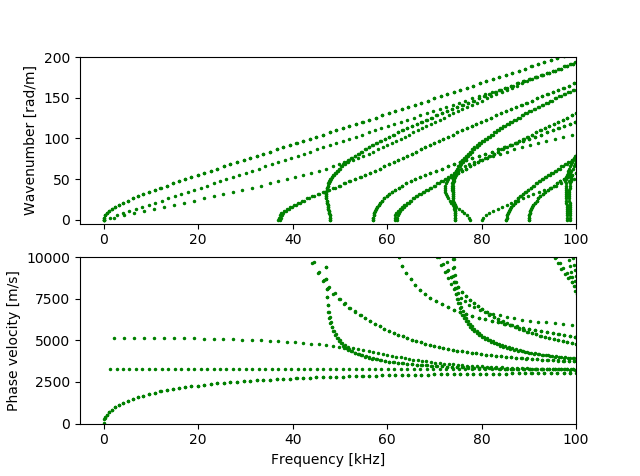
\includegraphics[width=14cm]{Zdjecia/5/wykres4}
\caption{Krzywe dyspersji otrzymane z wykorzystaniem elementów czworościennych dla stalowego pręta o promieniu 25mm.
Pozostałe parametry symulacji to num\_of\_circles = 8 oraz num\_of\_points\_at\_c1 = 8}
\label{fig:wykres4}
\end{figure}

\begin{figure}[h]
\centering
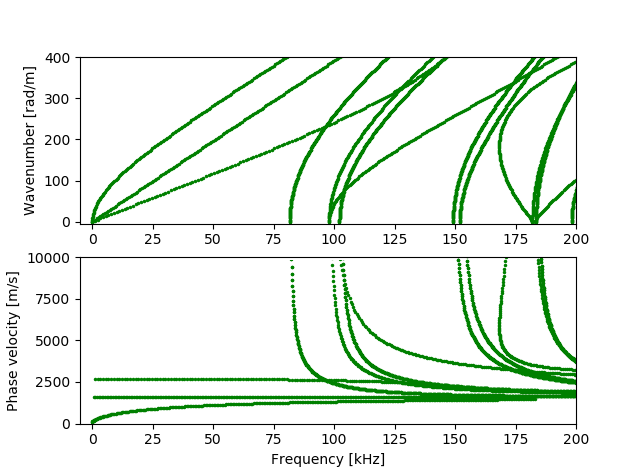
\includegraphics[width=14cm]{Zdjecia/5/wykres8}
\caption{Krzywe dyspersji otrzymane z wykorzystaniem elementów sześciennych dla stalowego pręta o promieniu 25mm.
Pozostałe parametry symulacji to firstCircle = 16, addNodes = 0, circles = 2}
\label{fig:wykres8}
\end{figure}


Wyniki różnią się do siebie częstotliwościami, w których pojawiają się kolejne postaci fali. Biorąc pod uwagę spodziewane wyniki, symulacja z wykorzystaniem elementów sześciennych wprowadza błąd na nieznanym etapie. Prędkości fali różnią się mocno od oczekiwanych.

W przypadku symulacji z elementami czworościennymi wyniki zbiegają do oczekiwanych wraz z zagęszczaniem siatki elementów. Przedstawia to rysunk \ref{fig:porownanie}. Widać na nim, że różnica pomiędzy wynikami z najrzadszą siatką, a wynikami ze średnią siatką, jest większa niż pomiędzy tą drugą, a siatką najgęstszą.  Na tej podstawie można wywnioskować, że obliczenia przebiegają poprawnie.

\begin{figure}[h]
\centering
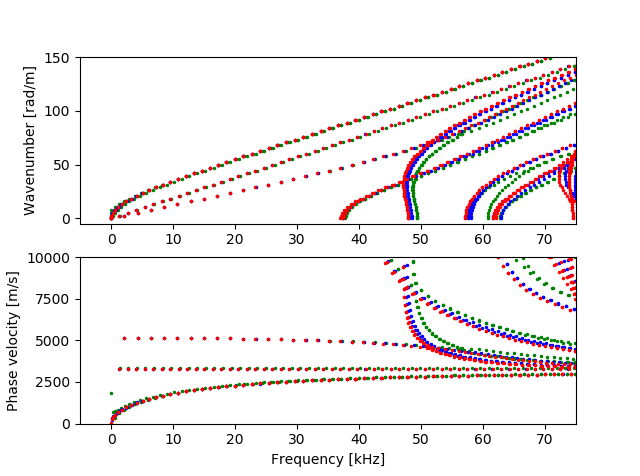
\includegraphics[width=14cm]{Zdjecia/5/porownanie}
\caption{Porównanie wyników z różną gęstością siatki. Kolor zielony - najrzadsza, niebieski - średnia, czerwony - najgęstsza}
\label{fig:porownanie}
\end{figure}

\subsection{Wyniki - sing-around}
\label{sec:53f}

Sekcja zawiera wyniki symulacji efektu sing-around dla sygnału chirp przedstawionego na rysunku \ref{fig:chirp}. Rysunek \ref{fig:fchirp} przedstawia widmo amplitudowe badanego sygnału. Krzywe dyspersji wykorzystane w symulacji są przedstawione w na rysunku \ref{fig:wykres4}, a za krzywe wzbudzalności posłużyły testowe krzywe eksponencjalne ukazane na rysunku \ref{fig:singExc}.

\begin{figure}[h]
\centering
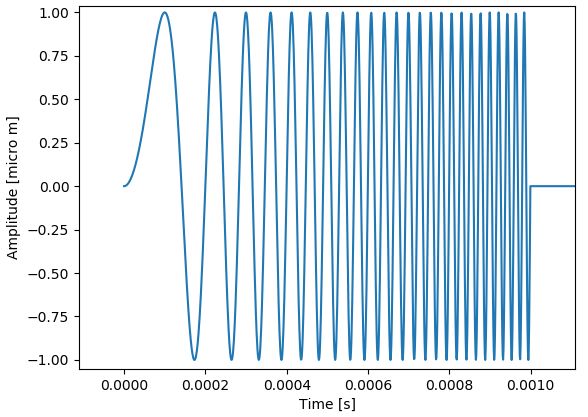
\includegraphics[width=10cm]{Zdjecia/5/chirp1}
\caption{Sygnał chirp}
\label{fig:chirp}
\end{figure}

\begin{figure}[h]
\centering
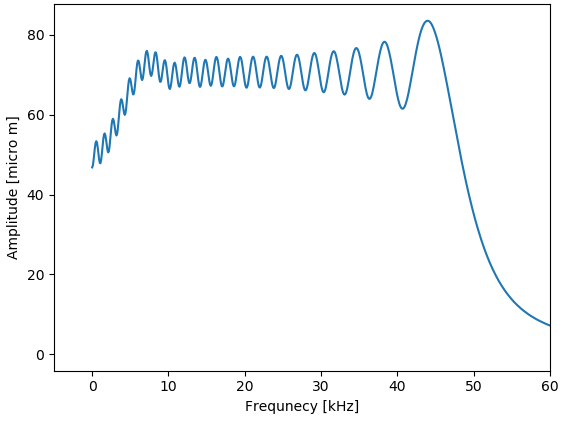
\includegraphics[width=10cm]{Zdjecia/5/chirp_widmo}
\caption{Widmo sygnał chirp}
\label{fig:fchirp}
\end{figure}

\begin{figure}[h]
\centering
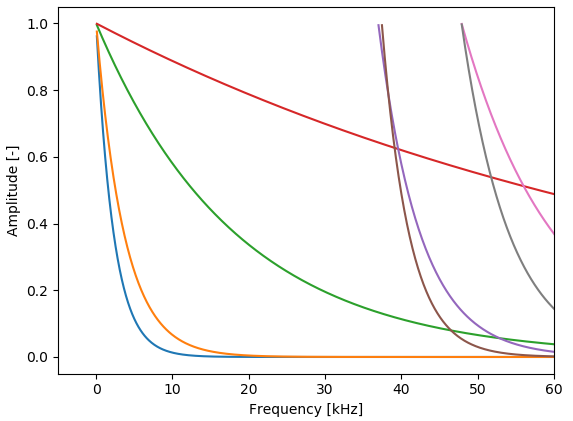
\includegraphics[width=10cm]{Zdjecia/5/krzywe_wzbudzalnosci}
\caption{Krzywe wykorzystane w roli krzywych wzbudzalności}
\label{fig:singExc}
\end{figure}

Rysunku \ref{fig:1prop} i \ref{fig:8prop} przedstawiają wyniki symulacji po 1 przejściu i po 8 kolejnych przejściach fali na długości 2 metrów.

\begin{figure}[h]
\centering
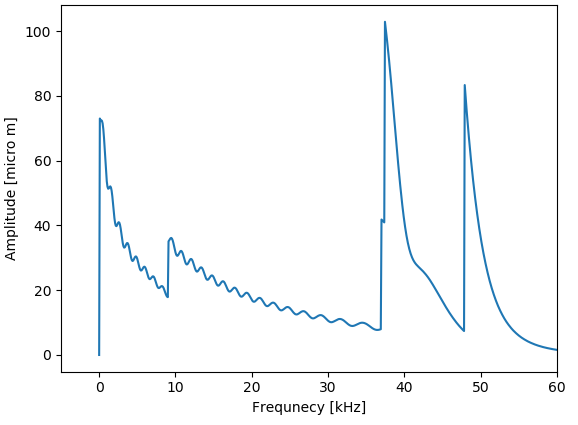
\includegraphics[width=10cm]{Zdjecia/5/1}
\caption{Widmo sygnału po jednym przejściu fali}
\label{fig:1prop}
\end{figure}

\begin{figure}[h]
\centering
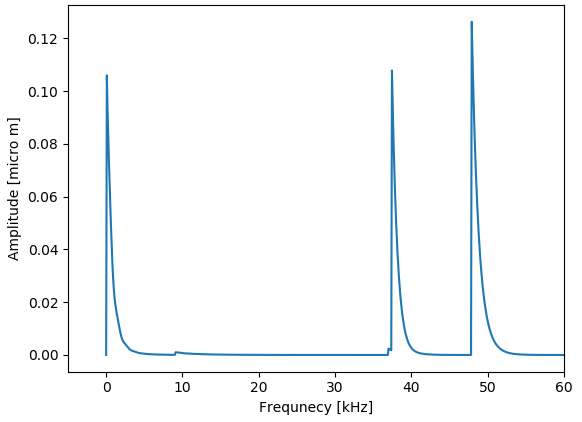
\includegraphics[width=10cm]{Zdjecia/5/8}
\caption{Widmo sygnału po ośmiu przejściach fali}
\label{fig:8prop}
\end{figure}

Przesunięcia fazowe sygnału nie powodują zmiany jego widma amplitudowego. Uwzględnienie krzywych wzbudzalności powoduje natomiast ukazanie się częstotliwości rezonansowych obiektu. Kolejne przejścia powodują, że częstotliwości rezonansowe są coraz bardziej uwidocznione.

Wykrywanie tego typu częstotliwości w sygnale ma duże zatosowanie w badaniu stanu konstrukcji. Problemem może się okazać dostosowanie czasu, w którym występują interesujące nas częstotliwości. Efekt dyspersji powoduje, że składowe o różnych częstotliwościach poruszają się z różnymi prędkościami, a co za tym idzie mogą się nakładać raz wzmacniając, a raz wygaszając.



